\chapter{Exceptions and Files}

\section{Exceptions}

Consider this program:

\begin{code}
import java.util.Scanner;

public class ErrorProne {

    public static void main(String[] args) {
        int[] data = {10, 66, 47, 11};
        
        Scanner input = new Scanner(System.in);
        
        System.out.print("Enter index 0-3: ");
        int index = input.nextInt();
        
        System.out.print("Enter number to divide by: ");
        int divisor = input.nextInt();
        
        int result = data[index] / divisor;
        System.out.printf("quotient of %d and %d is %d\n",
            data[index], divisor, result);
    }
}
\end{code}

If you enter a non-number the program crashes:

\begin{stdout}
Enter index 0-3: two
Exception in thread "main" java.util.InputMismatchException
	at java.base/java.util.Scanner.throwFor(Scanner.java:939)
	at java.base/java.util.Scanner.next(Scanner.java:1594)
	at java.base/java.util.Scanner.nextInt(Scanner.java:2258)
	at java.base/java.util.Scanner.nextInt(Scanner.java:2212)
	at ErrorProne.main(ErrorProne.java:11)
\end{stdout}
\index{stack trace}
The lines beginning with \texttt{at} are a {\em stack trace}. They show the chain of method calls in reverse chronological order with the file name and line number. You'll want to look for the one that is in your program. In this case, the error was in \texttt{ErrorProne.java:11}, where the \texttt{11} is the line number in the source file with the \java{nextInt} call.

If you enter an index outside the array bounds, the program crashes (the output has been reformatted to fit on the line length of this page):

\begin{stdout}
Enter index 0-3: 5
Enter number to divide by: 0
Exception in thread "main"
  java.lang.ArrayIndexOutOfBoundsException:
  Index 5 out of bounds for length 4
	at ErrorProne.main(ErrorProne.java:21)

\end{stdout}

And if you enter a zero as the divisor, you get yet another error:

\begin{stdout}
Enter index 0-3: 2
Enter number to divide by: 0
Exception in thread "main"
  java.lang.ArithmeticException: / by zero
    at ErrorProne.main(ErrorProne.java:21)
\end{stdout}

All of these errors are called {\em exceptions}---exceptional conditions after which the program cannot continue to run. In Java, we say that the program {\em throws} an exception when it fails.

You already know how to handle these problems before they crash your program: you can use an \java{if} statement with \java{Scanner}'s \java{hasNextInt} method to make sure that the user enters an integer. You can use \java{if} statements to check that the index number is between 0 and the array's length, and that the divisor is non-zero.

\index{\java{try}}
\index{\java{catch}}
In addition to using an \java{if} statement to avoid errors, Java has another general mechanism for catching exceptions before they stop your program:  \java{try} and \java{catch}.

Let's enclose the code that could have an error in a \java{try} block:

\begin{code}
try {
    System.out.print("Enter index 0-3: ");
    int index = input.nextInt();
    
    System.out.print("Enter number to divide by: ");
    int divisor = input.nextInt();
    
    int result = data[index] / divisor;
    System.out.printf("quotient of %d and %d is %d\n",
        data[index], divisor, result);
}
\end{code}

The \java{try} block is followed by a \java{catch} block that specifies the exception we want to handle
and how to handle it.  Let's start with the division by zero, which generated a \java{java.lang.ArithmeticException}:

\begin{code}
catch (ArithmeticException ex) {
    System.out.println("Number to divide by cannot be zero.");
}
\end{code}

If you recompile and run the program and enter \texttt{2} and \texttt{0} as your numbers, you'll get the error message in the \java{catch} block. Notice that the \java{printf} statement after the division doesn't occur---when an exception is thrown, execution imediately jumps to the \java{catch}.

If you enter \texttt{five} or \texttt{5} for the first input, you'll still get the \java{NumberFormatException} or \java{ArrayIndexOutOfBoundsException}.
 
You may follow a \java{try} block with as many \java{catch} blocks as you want. Let's add two more \java{catch} blocks to handle these other two errors:

\begin{code}
catch (NumberFormatException ex) {
    System.out.println("You must enter digits for numbers.");
}
catch (ArrayIndexOutOfBoundsException ex) {
    System.out.printf("Index must be in range 0-%d\n", data.length);
}
\end{code}

The variable in parentheses after \java{catch} is local to the \java{catch} block. This means you can use the same variable name in all the \java{catch} blocks, and, by convention, most programmers name it \java{ex}. (We will put it to use later in the chapter.)

When an exception occurs, Java goes through the \java{catch} blocks in the order that they appear in your program and finds the first one that applies. In the preceding example, we could have put the \java{catch} blocks in any order. However, the order does become important once we examine the hierarchy of exceptions.

\section{The Hierarchy of Exceptions}
\index{exceptions!hierarchy}
All exceptions descend from the \java{Exception} class\footnotemark. This list shows many of the most common exceptions you will encounter when learning Java; each category contains many other classes:

\footnotetext{\java{Exception} is a child of the \java{Throwable} class. Another child of \java{Throwable} is \java{Error}, which is used for serious, system-level problems. You will very rarely encounter one of these.}

\begin{itemize}
    \item \java{Exception}
        \begin {itemize}
            \item \java{IOException}
                \begin{itemize}
                    \item \java{FileNotFoundException}
                \end{itemize}
            \item \java{RunTimeException}
            \begin {itemize}
                \item \java{ArithmeticException}
                \item \java{IllegalArgumentException}
                    \begin{itemize}
                        \item \java{IllegalFormatException}
                        \item \java{InvalidParameterException}
                        \item \java{NumberFormatException}
                    \end{itemize}
                \item \java{IndexOutOfBoundsException}
                    \begin{itemize}
                        \item \java{ArrayIndexOutOfBoundsException}
                        \item \java{StringIndexOutOfBoundsException}
                    \end{itemize}
                \item \java{NullPointerException}
              \end{itemize}
    \end{itemize}
\end{itemize}

If you put a \java{catch} for a parent class {\em before} a \java{catch} for a child class, the parent class will catch the error.
Thus, in this code fragment:

\begin{code}
try {
    int n = 12 / 0;
}
catch (Exception ex) {
    System.out.println("Something unexpected occurred.");
}
catch (ArithmeticException ex) {
    System.out.println("You can't divide by zero.");
}
\end{code}

You will see the ``Something unexpected occurred.'' message.  For this reason, always \java{catch} the more specific (child) exception classes before you \java{catch} the more general (parent) exception classes.

\section{Using the Exception Variable}
\index{exception variable}
Let's say you \java{catch} the most generic \java{Exception} possible, or one that could have many possible causes, such as \java{FileNotFoundException}. How can you give the user more information than just ``something unexpected occurred''? You can use the variable that you declared in the \java{catch} clause. Here are some methods that you can use\footnotemark:

\footnotetext{These methods are from the \java{Throwable} class, which is the parent of all Java exceptions.}

\begin{description}
  \item[\texttt{getMessage()}] \hfill \\ Returns a detailed message string
  \item[\texttt{toString()}] \hfill \\ Returns a short description
  \item[\texttt{printStackTrace()}] \hfill \\ This \java{void} method prints the exception and its stack trace to the standard error stream, which is your terminal window
\end{description}

For example, you could \java{catch} {\em only} \java{Exception} and use one of these methods to tell users what went wrong:

\begin{code}
catch (Exception ex) {
    System.out.println("An error occurred:");
    System.out.println(ex.toString());
}
\end{code}

You can see this in action in file {\it ErrorProneGeneralException.java} in the code repository. As you can see, the error messages are not as satisfactory as those you would write yourself when handling the specific exceptions.

\section{The \java{finally} clause}
\index{\java{finally}}
Sometimes programs need to take an action whether the code in the \java{try} block succeeded or not. (For example, if you have allocated resources and want to ``clean up'' before exiting the program.) This is the role of the \java{finally} clause. It is executed whether the \java{try} block succeeded or an exception was caught by a \java{catch} block. In fact, it is executed even when there is a \java{return} or \java{break} in a block:

\begin{code}
public class FinallyTest {

    public static void main(String[] args) {
        Scanner input = new Scanner(System.in);
        
        try {
            int result = 17 / 5;
            System.out.printf("quotient of 17 and 5 is %d\n",
               result);
            return; // exits the main() method
        }
        catch (ArithmeticException ex) {
            System.out.println("You can't divide by zero.");
        }
        finally {
            System.out.println("In the finally clause.");
        }
        System.out.println("Does not print if return succeeds");
    }
}
\end{code}

This program will print \texttt{In the finally clause.} even though the \java{return} prevents the last \java{println} from happening.

\section{Throwing Exceptions}
Before proceeding, let's ask a philosophical question: why do these exceptions even exist? Why doesn't the JVM simply do something reasonable when it encounters one of these situations?  That's the whole problem---what does ``reasonable'' mean? For dividing by zero, some programs might want to return a zero as a default answer. Other programs might want to print an error message and end the program. Still others might want to detect the attempt to divide by zero and ask for new input.

Because the definition of ``reasonable'' is different for every program and every programmer, it makes sense for these exceptions that happen in many different circumstances to throw the problem back to the programmer and say, ``you handle this.'' 

If you are writing a library of Java methods for other people to use, you won't be able to anticipate all of your users' needs either. Your methods will also need to \java{throw} an \java{Exception} so that the people who use your methods can handle errors as they see fit.

For example, let's say you have a Java library with a method that calculates the average of an array of \java{double} values. If somebody hands you an empty array, that's an illegal argument, and you can write your code to \java{throw} an \java{IllegalArgumentException}:

\begin{code}
 1  public class ArrayStats {
 2    public static double average(double[] data) 
 3     throws IllegalArgumentException {
 4      int n = data.length;
 5      if (n > 0) {
 6        double sum = 0.0;
 7        for (double value: data) {
 8          sum += value;
 9        }
10        return sum / n;
11      } else {
12        throw new IllegalArgumentException("Empty array");
13      }
14    }
15  }
\end{code}

In line 3, specify that this method \java{throws} an \java{IllegalArgumentException}.

In line 12, when the length of the array is zero, use the keyword \java{throw} and create a \java{new} \java{IllegalArgumentException}. The argument to the constructor is the value that will be returned when someone calls
the exception's \java{getMessage} method.

Here's an example that calls the code (without \java{try} and \java{catch}) and the resulting error, formatted to fit the page:

\begin{code}
public class TestArrayStats {
    public static void main(String[] args) {
        double[] items = new double[0];
        double result = ArrayStats.average(items);
        System.out.println("Average is " + result);
    }
}

Exception in thread "main"
  java.lang.IllegalArgumentException: Empty array
        at ArrayStats.average(ArrayStats.java:12)
        at TestArrayStats.main(TestArrayStats.java:5)
\end{code}

If your method can throw more than one exception, you list them separated by commas in the \java{throws} clause:

\begin{code}
public static void example() throws IllegalArgumentException,
  ArithmeticException, NumberFormatException {
    // ...code
}
\end{code}

\section{Checked and Unchecked Exceptions}
\index{unchecked exceptions}
\index{exceptions!unchecked}

All of the exceptions used in the preceding examples (and all exceptions that are descendants of \java{RuntimeException}) are called {\em unchecked exceptions}. Java doesn't require you to enclose operations that cause such exceptions in a \java{try}-\java{catch} block. This is a good thing, or you'd need \java{try}-\java{catch} blocks around every division, array access, and string-to-numeric conversion.

For many operations that could throw an unchecked exception, you are better off using an \java{if} statement to avoid the error in the first place. You can, for example, use an \java{if} to check if an index is within array bounds, a divisor is non-zero, or if the user has actually entered data that can be converted to integer. This also gives you greater control over the program flow and structure. See, for example, the {\it NormalErrorChecking.java} file in the code repository.

\index{checked exceptions}
\index{exceptions!checked}

So, why are we talking about \java{try} and \java{catch} at all? Because there are some exceptions that can't easily be handled by an \java{if}-\java{else}. These exceptions are called {\em checked exceptions}. The Java compiler requires you to enclose operations that might throw these exceptions in a \java{try} block and provide a \java{catch} block to handle them. You are also required to list them in a \java{throws} clause if you are throwing those exceptions yourself. Foremost of these checked exceptions is the \java{IOException}, generated by I/O (Input/Output) operations. When you are working with files in Java, you will need to check this exception. This leads us to the next major topic in this chapter:

\section{Files}

Up to this point, you've entered all the data for a program from the keyboard, using a \java{Scanner} with \java{System.in}.  What if someone sends you a file of several months' worth of weather data from Munich, Germany, in a file named {\em klima.txt}. You can find this file in the {\em ch018} folder in the repository\footnotemark.

\footnotetext{The file is an edited version of the data at \url{https://opendata.dwd.de/climate_environment/CDC/observations_germany/climate/daily/kl/recent/tageswerte_KL_03379_akt.zip}}

\begin{stdout}
MESS_DATUM;TMK;TXK;TNK
20200106;0.8;6.0;-2.5
20200107;2.4;4.6;-2.1
20200108;3.6;7.2;-1.3
20200109;7.7;14.5;3.6
...
20210704;17.9;22.9;14.7
20210705;18.5;22.4;13.9
20210706;21.8;31.5;15.4
20210707;18.2;20.5;16.7
20210708;16.9;20.1;14.7
\end{stdout}

The columns stand for date, average daily temperature, high temperature, and low temperature (temperatures are in $^\circ$C).
If you want to find the maximum temperature and minimum temperature across the whole time period, you certainly don't want to have to type all the numbers again at the keyboard. Instead, you want Java to be able to read the file from your disk.

\subsection{The \java{File} Object}
In order to access a file, you must use its path name to create a \java{File} object. A path name describes how to get to a file in the file system. For this chapter, we’ll presume that your data files are in the same directory as the {\em .class} file for your program. That way, the path name is the same as the file name. (For more details about path names, see Appendix~\ref{pathnames}.)

The resulting object doesn't give you access to the file contents; rather, it gives you access to information about the file.

Here's the start of a program that lets you enter a path name and find out about that file:

\begin{code}
import java.util.Scanner;
import java.io.File; // this is a new import

public class FileInfo {
    public static void main(String[] args) {
        Scanner input = new Scanner(System.in);
        System.out.print("Enter a path name: ");
        String pathName = input.nextInt();
        
        File f = new File(pathName);
\end{code}

The variable \java{f} is what, in other programming languages, is called a {\em file handle} or {\em file descriptor}. The code continues by calling some of the more useful methods in the \java{File} class:

\begin{code}
        System.out.println("File exists: " + f.exists());
        System.out.println("File size:   " + f.length());
        System.out.println("Readble:     " + f.canRead());
        System.out.println("Writeable:   " + f.canWrite());
        System.out.println("Executable:  " + f.canExecute());
        System.out.println("Directory:   " + f.isDirectory());
        System.out.println("Normal file: " + f.isFile());
        System.out.println("Hidden file: " + f.isHidden());
    }
}
\end{code}

A couple of notes: the \java{length} method returns the file size in bytes. It is possible for a file to be neither a directory nor a ``normal file''---the \texttt{/dev/zero} path on Linux refers to a {\em virtual file} that is neither.

The \java{File} class also has methods that let you delete files, rename them, and create directories. For details, see \url{https://docs.oracle.com/en/java/javase/16/docs/api/java.base/java/io/File.html}.

\subsection{Reading Files}

Let's write a program that opens the {\em klima.txt} file and finds the maximum and minimum daily temperature across the time period described in the file.

In order to read the contents of a file, you must open a \java{Scanner} based on the \java{File} object. But if you try code like this:

\begin{code}
import java.util.Scanner;
import java.io.File;

public class LineCount {

    public static void main(String[] args) {        
        File f = new File("klima.txt");
        
        Scanner input = new Scanner(f);
    }
}
\end{code}

The compiler will complain (message reformatted to fit page width):

\begin{stdout}
Klima.java:9: error: unreported exception
FileNotFoundException; must be caught or declared to be thrown
        Scanner input = new Scanner(f);
                        ^
1 error
\end{stdout}

The \java{FileNotFoundException} is a {\em checked exception}, and the compiler insists that you either catch it or throw it to the caller.

This will require you to import \java{java.io.FileNotFoundException} and set up a \java{try}-\java{catch} block. 

\begin{code}
import java.util.Scanner;
import java.io.File;
import java.io.FileNotFoundException;

public class Klima {

    public static void main(String[] args) {        
        File f = new File("klima.txt");
        try {
            Scanner input = new Scanner(f);
            // code goes here
            input.close();
        }
        catch (FileNotFoundException ex) {
            System.out.println("Can't find file klima.txt");
        }
    }
}
\end{code}

Now we are set to read the file's contents. Rather than write the whole program right now, let's start by reading the file one line at a time, printing them out to the screen, and counting the number of lines. Here's the code that goes inside the \java{try} block. The \java{hasNextLine} method returns \java{false} when it hits the end of the file:

\begin{code}
            while (input.hasNextLine()) {
                String oneLine = input.nextLine();
                System.out.println(oneLine);
                lineCount++;
            }
            System.out.println("# of lines: " + lineCount);
            input.close();
\end{code}

Now, that we know that we can sucessfully open and read the file, we can modify the code to accomplish the task we want to do: finding the minimum and maximum temperatures.

The program will read lines one at a time and then extract the data from each line. Because \java{Scanner}'s \java{next} and \java{nextDouble} methods use whitespace to separate items, we can't use them ``as-is'' here, where data items are separated by semicolons. We could solve this problem by using the \java{useDelimiter} method to change the separator to a semicolon, but that would deprive us of the opportunity to learn about a new \java{String} method and practice more with exceptions.

Let's replace the line-counting code with this code for finding the maximum and minimum temperatures:

\begin{code}
double max = -1000.0;
double min = 1000.0;
String[] items = oneLine.split(";");
if (items.length == 4) {
    dayMax = Double.parseDouble(items[2]);
    dayMin = Double.parseDouble(items[3]);
    if (dayMax > max) {
        max = dayMax;
    }
    if (dayMin < min) {
        min = dayMin;
    }
}
\end{code}

The new \java{String} method is \java{split}. Given a delimiter, this method splits the given \java{String} into an array of strings wherever it finds the delimiter that you give it as an argument. For example, after this code executes:

\begin{code}
String s = "sister-in-law";
String[] parts = s.split("-");
\end{code}

The \java{parts} array will be \java{\{"sister", "in", "law"\}}.

Similarly, the program uses \java{oneLine.split(";")} to separate the items on each line. If there aren't four items on a line, it's incomplete, and the program does nothing (effectively skipping over the line).

We now have a problem: the first line doesn't have any numbers on it, and trying to use \java{parseDouble} on the titles will throw a \java{NumberFormatException}. One way to solve the problem is to read in the first line before entering the \java{while} loop and discarding the result. Another way to solve this problem (which could also occur if the file we were given had bad data in it), is to use another \java{try}-\java{catch}:

\begin{code}
try {
    double dayMax = Double.parseDouble(items[2]);
    double dayMin = Double.parseDouble(items[3]);
}
catch (NumberFormatException ex) {
    System.out.println("Ignoring non-numeric data "
        + ex.getMessage());
}
\end{code}


\subsection{Writing Files}

There are many Java classes for reading files. In this book, we've been using \java{Scanner} to read input because it contains many methods to make getting input simple.

In a similar way, there are many Java classes for writing files. We'll discuss only one of them: \java{PrintWriter}. To use this class, you must:

\begin{code}
import java.io.PrintWriter;
\end{code}

Just as you created a \java{Scanner} by using a \java{File} object as a parameter to the constructor, you can write to a disk file by creating a \java{File} object with the path you want and then use that object as a parameter to the \java{PrintWriter} constructor. And, just as the compiler required you to enclose the code in a \java{try}-\java{catch} block, you must do the same when opening a \java{PrintWriter}

\begin{code}
File f = new File("output.txt");
try {
    PrintWriter output = new PrintWriter(f);
    // code to write to file goes here
}
catch (FileNotFoundException ex) {
    System.out.println("Unable to open output file.");
}
\end{code}

Just like \java{System.out}, the \java{PrintWriter} object \java{output} we have created has \java{print}, \java{println}, and \java{printf} methods. Instead of writing to your screen, they write data to the file you specified.

\subsection {Writing Files - Two Important Notes}

\begin{enumerate}
\item When you open a \java{PrintWriter} to a \java{File} that does not exist, it will be created for you. If you open a \java{PrintWriter} to a \java{File} that {\em does} exist, {\bf the existing file will be deleted and re-created}. Any information that was in the file will be gone, even if you never write anything to the \java{PrintWriter}.

This means that it is always useful to use the \java{exists} method to check if a file already exists and, when possible, give the user the option to overwrite the old file or exit the program.

\item When you do a \java{println} to a \java{PrintWriter}, the data is not written to disk immediately. Instead, it is kept in a {\em buffer}, and is written only when the buffer is full. If you exit the program with the buffer partially filled, there is a chance that it might not be written to disk. {\em Always} call the \java{close} method on your output files to make sure that the buffer is written to disk.

If you run this program:

\begin{code}
import java.io.File;
import java.io.FileNotFoundException;
import java.io.PrintWriter;

public class PartialWrite {

    public static void main(String[] args) {        
        File f = new File("write_test.txt");
        try {
            PrintWriter output = new PrintWriter(f);
            output.println("Example of writing to a file.");
            // output.close(); // uncomment this line 
        }
        catch (FileNotFoundException ex) {
            System.out.println("Can't open file write_test.txt");
        }
    }
}
\end{code}

without closing the file, the resulting {\em write\_test.txt} file will be empty.
If you uncomment the \java{output.close();} line and run the program again, the file will contain the output.
 
\end{enumerate}

\section{\java{try} with Resources}

Because it is important to close files, Java has a syntax for associating \java{File}s with input and output classes as part of the \java{try} syntax. When using this syntax, the Java Virtual Machine will automatically close the input and output when the \java{try} block exits. Here is an example that uses \java{try} with resources to open  a \java{PrintWriter}:

\begin{code}
File outFile = new File("output_path.txt");
try (PrintWriter outWriter = new PrintWriter(outFile)) {
    outWriter.println("Example of try with resources.");
}
catch (FileNotFoundException ex) {
    System.out.println("Error: " + ex.getMessage);
}
\end{code}

The declaration of \java{outWriter} is now in parentheses after \java{try} rather than after the block's opening brace.
We no longer need to call \java{outWriter.close()}---the JVM will automatically do the call when it exits the \java{try}-\java{catch} block.

You can declare as many input and output objects as you want inside the parentheses:

\begin{code}
File inFile = new File("input_path.txt");
File outFile = new File("output_path.txt");
try (
    Scanner inScan = new Scanner(inFile);
    PrintWriter outWriter = new PrintWriter(outFile);
) {
    // code...
}
catch (Exception ex) {
    // error handling...
}
\end{code}

The \java{File} declarations cannot go inside the parentheses; the compiler won't let you do that.

\section{Exercises}

\begin{exercise}
Write a program named {\em TestAverages.java} that asks the user for the name of an input file that has people's names and test scores. Each line has the person's name, a colon, and a list of scores separated by commas.

Next, the program asks the user for the name of an output file. The program will then read the input file and write a new output file with the names and their average scores, including the number of tests on which it is based.

Your program has to do the following error handling:

\begin{itemize}
\item If the input file does not exist or cannot be opened, print an appropriate error message.
\item If the output file cannot be opened, print an appropriate error message.
\item If an input line has a non-numeric entry for a score, print an error message to the screen with the bad data and skip that score.
\item If an input line has no scores, print an appropriate message to the screen.
\end{itemize}

% For this input file {\em sampleScores.txt}:

\begin{stdout}
Juan Fulano: 88, 82, 89
Tran Thi B: 91, 87.5, 92, 89, 88.5
Jan Kovacs: 91, 93, 8r, 74.5
Joseph Schmegeggie:
Erika Mustermann: 79.5, 83.5, 90, 92
\end{stdout}

Here is the result of running the program several times. First, with a bad input file name:

\begin{stdout}
Enter input file name with test scores: nosuchfile.txt
Cannot find input file nosuchfile.txt
\end{stdout}

With a good input file name but a bad output file name. Notice that the message tells why the output file failed:

\begin{stdout}
Enter input file name with test scores: sampleScores.txt
Enter output file name for averages: /usr/output.txt
IO Error: /usr/output.txt (Permission denied)
\end{stdout}

With a good input and output file name:

\begin{stdout}
Enter input file name with test scores: sampleScores.txt
Enter output file name for averages: output.txt
Ignoring bad number  8r for Jan Kovacs
No numbers found on line Joseph Schmegeggie:
File output.txt written successfully.
\end{stdout}

After the program finishes successfully, the {\em output.txt} file looks like this:

\begin{stdout}
Juan Fulano: 86.33 (3 tests)
Tran Thi B: 89.60 (5 tests)
Jan Kovacs: 86.17 (3 tests)
Erika Mustermann: 86.25 (4 tests)
\end{stdout}

Some hints:

\begin{itemize}
\item Do not presume that the input file will always be named {\em sampleScores.txt} or the output file will always be named {\em output.txt}---the user gets to decide those names, not you!
\item  If a person has scores, but none of them are numeric, then they will have no tests to average. Your program needs to handle that situation correctly.
\item Use the \java{split} method in the \java{String} class to separate the name from the scores, and use it again to separate the individual scores. You will need to convert the resulting strings to \java{double}. Do this by using the \java{Double.parseDouble} method, which throws a \java{NumberFormatException} if given a non-numeric string as its parameter.
\end{itemize}

\end{exercise}

\begin{exercise}
Are you tired of having to write all the getter and setter methods when you create a new \java{class}? In this exercise, your program will ask for the name of a file that contains Java declarations, like this:

\begin{stdout}
public int age;
private double[] weights;
\end{stdout}

It will then ask for an output file name and create that file with the getters and setters:

\begin{stdout}
public int getAge() {
    return age;
}

public void setAge(int age) {
    this.age = age;
}

public double[] getWeights() {
    return weights;
}

public void setWeights(double[] weights) {
    this.weights = weights;
}
\end{stdout}

You may presume that the input file is formatted as follows:

\begin{enumerate}
\item Each line will begin with either \java{public} or \java{private}, without leading blanks.
\item The data type does not contain any blanks.
\item There is only one blank between the items on a line, and the data type does not contain any blanks. (These three items allow you to do \java{string.split(" ")} to get the individual parts of the declaration.)
\item Each line always ends with a semicolon.
\end{enumerate}

If the input file has blank lines, ignore them.

As in the preceding exercise, use exception handling to make sure that:

\begin{itemize}
\item If the input file does not exist or cannot be opened, print an appropriate error message.
\item If the output file cannot be opened, print an appropriate error message.
\end{itemize}

Hint: You can use the \java{replaceAll} method in the \java{String} class to get rid of the semicolon. The \java{replaceAll} method takes two parameters: a pattern to look for and a replacement string. For example, to replace all occurrences of \java{"ab"} with the empty string \java{""}:

\begin{code}
String original = "abracadabra";
String result = original.replaceAll("ab", "");
// result will be "racadra"
\end{code}

\end{exercise}

\begin{exercise}
In this exercise, you will consolidate data from one file to create another file in a program named {\em Consolidate.java}. The original data is in file {\em ch18/wildfires\_jan\_2015.txt} and was extracted from a database of 1.8 million wildfires from 1992 to 2015.\footnotemark

\footnotetext{Short, Karen C. 2017. Spatial wildfire occurrence data for the United States, 1992-2015 [FPA\_FOD\_20170508]. 4th Edition. Fort Collins, CO: Forest Service Research Data Archive. \url{https://doi.org/10.2737/RDS-2013-0009.4}}

Each line in the file contains:
\begin{itemize}
\item the year
\item the day of the year (1-365) the fire was discovered
\item fire perimeter (acres)
\item cause of fire (1 = lightning, 7 = arson, anything else is ``other'')
\end{itemize}

The first few lines of the file look like this:

\begin{stdout}
2015,1,2,2
2015,1,0,2
2015,1,1,2
2015,1,0,3
2015,1,0,3
2015,1,3,4
2015,1,0,4
\end{stdout}

Your program will read this file and create a new file where each line contains, separated by commas:

\begin{itemize}
\item The year
\item The day of year
\item The number of lightning-caused fires and their total acreage
\item the number of arson-caused fires and their total acreage
\item The number of fires with other causes and their total acreage
\end{itemize}

The first few lines of the output file look like this:

\begin{stdout}
2015,1,0,0,2,3,57,260
2015,2,2,1,1,0,35,13
2015,3,1,0,3,1,26,123
2015,4,0,0,2,33,21,255
\end{stdout}

Your program will read the input and output file names from the command line, so it could be invoked as follows:

\begin{stdout}
java Consolidate wildfires_jan_2015.txt wildfire_summary.txt
\end{stdout}

If the user gives too many or too few command line arguments, give an appropriate ``usage'' message.
Your program should give an appropriate message if the input file cannot be opened or the output file cannot be created.
As in the preceding exercise, use \java{split} to separate the items, and check that data can be converted to \java{double} by \java{catch}ing \java{NumberFormatException}.
\end{exercise}

\begin{exercise}

In this exercise, you will write two classes: a class that represents information about a city and a main program that processes that information. You can find some pseudocode for this exercise that may help you get the program organized and started in the repository, file {\em ch18/CityInfo\_Pseudocode.java}.

{\large\bf{The \java{City} class}}

First, write the \java{City} class that defines an object with these properties:

\begin{itemize}
    \item \java{private String country}: the two-letter country code
    \item \java{private String name}: the city name
    \item \java{private int population}: the city's population
\end{itemize}

Implement these methods:

\begin{description}
    \item [\texttt{public City(String country, String name, int population)}] \hfill \\ The constructor
    \item Accessors and mutators \hfill \\ Write an accessor (getter) and mutator (setter) for the population, and only a getter for the country code and city name; once the object is constructed, the country and city name never change. These must be \java{public}.
    \item [\texttt{public String toString()}] \hfill \\ Returns a string giving the country name, city name, and population, separated by semicolons.
\end{description}

Figure~\ref{fig.ch18.cityUML} shows a UML diagram for the \java{City} class.

\begin{figure}[!h]
\begin{center}
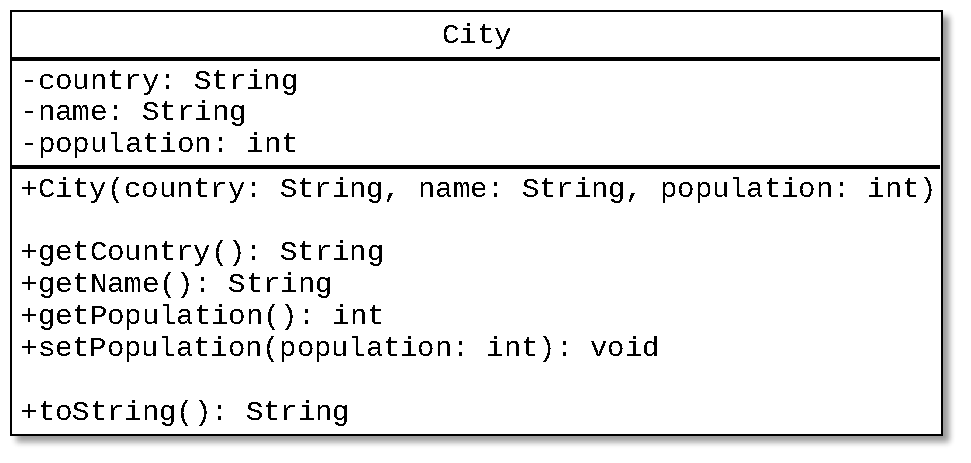
\includegraphics[scale=0.75]{figs/ch18/city.pdf}
\caption{UML diagram showing attributes and methods of the City class}
\label{fig.ch18.cityUML}
\end{center}
\end{figure}


{\large\bf{The \java{CityInfo} class}}

Then, write a class named \java{CityInfo} that contains the \java{main()} method.Use the {\em citylist.dat} file\footnotemark to set up the initial list of cities. The file is available from the repository at {\em ch18/citylist.dat} Each line of the text file has a country code, city name, and population, separated by semicolons. Your program must first read the city data file with this method:

\footnotetext{The data for this exercise came from \url{http://geonames.org/}, licensed under a Creative Commons Attribution 4.0 License (see \url{https://creativecommons.org/licenses/by/4.0/})}

\begin{stdout}
public static ArrayList<City> readCityFile(String fileName)
\end{stdout}

This method will open the given \java{fileName}, read it, and return an \java{ArrayList} of \java{City} objects corresponding to each line of the file.

If a line in the file has bad data (non-numeric population or too many or too few entries), your program will print an error that displays the bad line without entering any new data into the \java{ArrayList}. The \java{citylist.dat} file in the repository purposely contains some lines with bad data so you can test to see if your error-handling code works. Do not write your code for this specific file; another person's file might have bad data on different lines with different data on them.

If the file does not exist, the method prints an appropriate error message and returns an empty \java{ArrayList<City>}.

If the returned \java{ArrayList} is not empty, the program will repeatedly ask for a country code (or ENTER to quit).
Once the user enters a country code, the \java{main()} method will call this method:

\begin{stdout}
public static int statistics(String countryCode,
   ArrayList<City> cityList)
\end{stdout}

The \java{statistics()} method will go through the city list and

\begin{itemize}
    \item Calculate the total number of cities in the given country.
    \item If there are more than zero cities:
        \begin{itemize}
            \item Print the total number of cities
            \item Print the average population for those cities
        \end{itemize}
    
    \item Otherwise, prints an appropriate error message.
    \item Returns the total number of cities found.
\end{itemize}

The \java{main()} method will then use this returned value. If it is greater than zero, you will write a new file name {\em CC.dat}, where {\em CC} stands for a country code. This file will have the information for the cities in that country in the same format as \java{citylist.dat}. For example, if the country code is \java{JP}, your program will create a file named {\em JP.dat}. You will use a method named

\begin{stdout}
public static void writeCountryFile(String countryCode,
    ArrayList<City> cityList)
\end{stdout}

to do this. If there is an \java{IOException} while opening the output file or writing the data, print an appropriate error message. You must use the exception's \java{getMessage()} method when constructing your error message. If the file is written successfully, print a message letting the user know that the file has been created. This message {\em must} contain the file name.

{\large\bf{Handling Exceptions}}

Your program must handle these exceptions:

\begin{itemize}
    \item Catch \java{FileNotFoundException}when opening a \java{Scanner} for the input file. You could use the \java{File.exists()} method, but let's use exceptions to get more practice.)
    \item Catch \java{NumberFormatException} when reading the input file and converting strings to numbers.
    \item You will probably need nested \java{try}/\java{catch} blocks for file input: one outside the read loop when opening the file, and one inside the read loop to skip badly formatted lines.
    \item Catch \java{IOException} when writing an output file.
\end{itemize}

Here are some things to note:

\begin{itemize}
    \item You must accept input in either upper or lower case.
    \item You will need to loop through the \java{cityList} twice; once in \java{statistics()} to get the total and average (if applicable), and again in \java{writeCountryFile()} to create the output file. This is a design decision---I decided these are two separate tasks to be done by two methods, rather than combining both tasks into one method.
\end{itemize}

Here is what the program output might look like. Your output does not have to look exactly like this, but it must reflect the same information.

\begin{stdout}
Reading city file...
"AB;Too few" does not have three entries.
"CD;Too many;1056382;extra" does not have three entries.
"EF;Bad number;one million" does not have a number on it.

Enter a two-letter country code, or press ENTER to quit: UA
Number of cities in UA: 5
Average population is 1,457,504.
File UA.dat written successfully.
Enter a two-letter country code, or press ENTER to quit: LU
No cities found in LU.
Enter a two-letter country code, or press ENTER to quit: MX
Number of cities in MX: 11
Average population is 2,427,622.
File MX.dat written successfully.
Enter a two-letter country code, or press ENTER to quit: 
\end{stdout}

Here are the contents of the file {\em UA.dat}

\begin{stdout}
UA;Kiev;2797553
UA;Kharkiv;1430885
UA;Dnipropetrovsk;1032822
UA;Donets'k;1024700
UA;Odessa;1001558
\end{stdout}

Here is an example of the output you might get for an error while writing the file (I deliberately caused this error by changing my directory to be read-only).

\begin{stdout}
Error writing FR.dat
FR.dat (Permission denied)
\end{stdout}

\end{exercise}

\begin{exercise}
In this exercise, you will write two classes: a class that represents a bank account and a program that works like an ATM for bank accounts. The code repository has some pseudocode in file {\em ch18/ATM\_Pseudocode.java} that may help you get the program organized and started. 

{\large\bf{The \java{Account} class}}

First, create an \java{Account} class. An \java{Account} object has these properties:

\begin{itemize}
    \item \java{private int acctNumber}: the account number
    \item \java{private String name}: the account holder's name
    \item \java{private double balance}: the current balance in the account
\end{itemize}

Implement these methods:

\begin{description}
    \item[\texttt{public Account(int acctNumber, String name, double balance)}] \hfill \\ The constructor
    \item[\texttt{public String toString()}] \hfill \\  Returns a string giving the account ID, name, and balance, separated by colons. Do not use \java{format()} on the balance; you want to keep the number as accurate as possible.
    \item[\texttt{public void deposit(double amount)}] \hfill \\  Adds the given amount to the current balance. If the amount is negative, the balance must not be changed; otherwise, the \java{balance} property is updated to reflect the deposit.
    \item[\texttt{public void withdraw(double amount)}] \hfill \\ Withdraws the given amount from the current balance. If the amount is negative or greater than the current balance, the balance must not be changed; otherwise, the \java{balance} is updated to reflect the withdrawal.
\end{description}

You must also write a getter and setter for the balance, and only a getter for the name and account number; once the account is constructed, the name and account number never change. The getters and setters must be \java{public}.

Note that \java{deposit()} and \java{withdraw()} do not print error messages if they get incorrect input; they simply ignore it. It is up to the program that calls these functions to provide the error messages for the user of the program.

{\large\bf{The \java{Customer} class}}

Next, write a program named \java{Customer.java} that has a \java{main()} method. This class provides an ``ATM''-like interface to a set of bank accounts. Use the following {\em accounts.dat} file to set up the initial set of accounts. Each line of the text file has an account ID, name, and starting balance, separated by colons. Your program must first read the account data file and build an \java{ArrayList} of \java{Account} objects corresponding to each line. If the file does not exist, your program must output a reasonable error message and then quit.

\begin{stdout}
15725:Christina Plaka:456.71
23981:Roz Chast:1853.22
57012:Georges Remi:3571.85
46287:Raquel Corcoles:783.00
31954:Eiichiro Oda:854.02
84373:Scott McCloud:2733.96
\end{stdout}

If the file is read successfully, the program will repeatedly ask for an account number (or ENTER to quit). This is equivalent to inserting an ATM card. Repeat until the account number is valid. Hint: write a method like this:

\begin{stdout}
public static int findIndex(ArrayList<Account> accountList,
   int accountNumber)
\end{stdout}

This method will go through the \java{accountList} and return the index of the account with the given \java{accountNumber}, or -1 if the account number does not belong to any of the accounts in the array.

Print a message that greets the customer by name. Then repeatedly ask the customer if they want to deposit, withdraw, or finish the transactions.

\begin{itemize}
    \item If the customer wishes to deposit, ask for the amount until you get a number greater than or equal to zero; then perform the transaction and display the balance. Print an appropriate message for invalid input. You must handle exceptions here.
    \item If the customer wishes to withdraw, ask for the amount until you get a number greater than or equal to zero and less than or equal to the current balance; then perform the transaction and display the balance. Print an appropriate message for invalid input. You must handle exceptions here.
    \item If the customer is finished, print a message to say goodbye to the customer, write the entire account array back to disk, and return to the account number prompt. (This is equivalent to giving the customer their card back).
\end{itemize}

This program must print all monetary amounts preceded by a dollar sign and with two digits after the decimal point. This is where you {\em do} want to use \java{format} to round to two decimal places.

{\large\bf{Handling Exceptions}}

Your program must handle exceptions when opening the {\em accounts.dat} file. It must produce a reasonable error message and quit rather than crashing if the file doesn't exist.

Your program must also handle exceptions if the user enters invalid input such as``fifteen'' for the account number or amount to deposit/withdraw.

The exceptions you will probably want to use the most are \java{java.IO.IOException} for file errors and \java{NumberFormatException} for invalid numbers.

Here is what you might see as output when you run your program:

\begin{stdout}
Enter your account number: 12345
Unknown account number
Enter your account number: five
five is not a number
Enter your account number: 57012
Hello, Georges Remi!
Your current balance is $3571.85
D)eposit, W)ithdraw, or F)inish? D
Enter amount to deposit: $-20
You cannot deposit a negative amount.
D)eposit, W)ithdraw, or F)inish? D
Enter amount to deposit: $fifty
fifty is not a valid number.
D)eposit, W)ithdraw, or F)inish? D
Enter amount to deposit: $50
Your current balance is $3621.85
D)eposit, W)ithdraw, or F)inish? w
Enter amount to withdraw: $-200
You cannot withdraw a negative amount.
D)eposit, W)ithdraw, or F)inish? w
Enter amount to withdraw: $570.00
Your current balance is $3051.85
D)eposit, W)ithdraw, or F)inish? f
Goodbye, Georges Remi.

Enter your account number: 23981
Hello, Roz Chast!
Your current balance is $1853.22
D)eposit, W)ithdraw, or F)inish? w
Enter amount to withdraw: $1890
You cannot withdraw more than you have.
D)eposit, W)ithdraw, or F)inish? w
Enter amount to withdraw: $80
Your current balance is $1773.22
D)eposit, W)ithdraw, or F)inish? f
Goodbye, Roz Chast.

Enter your account number:
ATM program concludes.
\end{stdout}

After you finish running this program, the {\em accounts.dat} file will have the new balance(s):

\begin{stdout}
15725:Christina Plaka:456.71
23981:Roz Chast:1773.22
57012:Georges Remi:3051.85
46287:Raquel Corcoles:783.0
31954:Eiichiro Oda:854.02
84373:Scott McCloud:2733.96
\end{stdout}

\end{exercise}
